\documentclass[11pt,oneside,a4paper]{article}
\usepackage{graphicx}
\usepackage{booktabs}
\usepackage{caption}
\usepackage{subcaption}
\usepackage{amsmath}
\usepackage{amsfonts}
\usepackage{amssymb}
\usepackage{lscape}
\usepackage{psfrag}
\usepackage[usenames]{color}
\usepackage{bbm}
\usepackage[update]{epstopdf}
\usepackage[bookmarks,pdfstartview=FitH,a4paper,pdfborder={0 0 0}]{hyperref}
\usepackage{verbatim}
\usepackage{listings}
\usepackage{textcomp}
\usepackage{course}
\usepackage{fancyhdr}
\usepackage{multirow}
\pagestyle{fancy}
\usepackage{tikz}
\usepackage{subcaption} 
\usepackage{float}


\renewcommand{\sectionmark}[1]{\markboth{#1}{#1}}
\renewcommand{\subsectionmark}[1]{\markright{#1}}

\fancyhf{}
\fancyhead[RO]{\nouppercase{\footnotesize\sc\leftmark\ \hrulefill\ \thepage}}
\fancyhead[RE]{\nouppercase{\footnotesize\sc\thepage\ \hrulefill\ }}
\renewcommand{\headrulewidth}{0pt}

\makeatletter
\def\cleardoublepage{\clearpage\if@twoside \ifodd\c@page\else%
\hbox{}%
\thispagestyle{empty}%
\clearpage%
\if@twocolumn\hbox{}\clearpage\fi\fi\fi}
\makeatother


\renewcommand{\topfraction}{0.9}  % max fraction of floats at top
\renewcommand{\bottomfraction}{0.8} % max fraction of floats at bottom
% Parameters for TEXT pages (not float pages):
\setcounter{topnumber}{2}
\setcounter{bottomnumber}{2}
\setcounter{totalnumber}{4}            % 2 may work better
\setcounter{dbltopnumber}{2}           % for 2-column pages
\renewcommand{\dbltopfraction}{0.9}    % fit big float above 2-col. text
\renewcommand{\textfraction}{0.07}     % allow minimal text w. figs
% Parameters for FLOAT pages (not text pages):
\renewcommand{\floatpagefraction}{0.7}  % require fuller float pages
% N.B.: floatpagefraction MUST be less than topfraction !!
\renewcommand{\dblfloatpagefraction}{0.7} % require fuller float pages

\sloppy

\widowpenalty=10000
\clubpenalty=10000

\edef\today{%\number\day\
\ifcase\month\or
January\or February\or March\or April\or May\or June\or July\or
August\or September\or October\or November\or December\fi\ \number\year}
\title{\vspace*{40.0mm}
  \bf\sf Support Vector Machine Assignment 
         \vspace*{20.0mm} \\
  \vspace*{40.0mm}
  %\vspace{-20mm}\framebox{DRAFT VERSION}\vspace{20mm} \\
  }
\author{\sf Mohamedhakim Elakhrass}
\date{\sf 15/07/2016}




\begin{document}

	
	
\begin{figure}
  \parbox[t]{125mm}{
    \vspace*{6mm}
    \scriptsize\sf           FACULTY OF BIOSCIENCE ENGINEERING\\
    \scriptsize\sf           Masters of Bioinformatics \\
    \scriptsize\sf\bfseries  Support Vector Machines \\}
  \parbox[t]{40mm}{
    \begin{flushright}
      \includegraphics[height=15mm]{logo.eps}
    \end{flushright}}
\end{figure}

\maketitle
\thispagestyle{empty}
\raggedbottom

\cleardoublepage
\pagenumbering{roman}
\setcounter{tocdepth}{2}
\tableofcontents
\cleardoublepage
\pagenumbering{arabic}

\cleardoublepage

\section{Assignment 1}
\subsection{Objectives}
The objectives of this assignment are to learn and work with real life applications of SVM. 
\subsection{Simple 2 Gaussian}
This sections looks at two simulated datasets. The datasets are created using the MatLab $randn()$ function. One dataset is centered around (1,1) and the other (-1,1)\\

\begin{figure}[H]
	\setbox0\hbox{%
		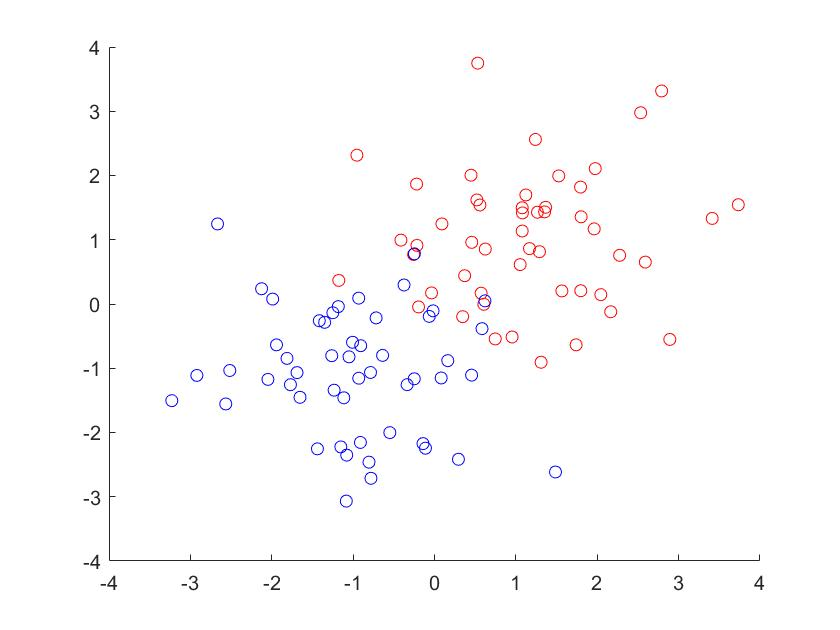
\includegraphics[width=.45\textwidth]{../Figures/2_Gaussians}%
	}%
	\setbox2\hbox{%
		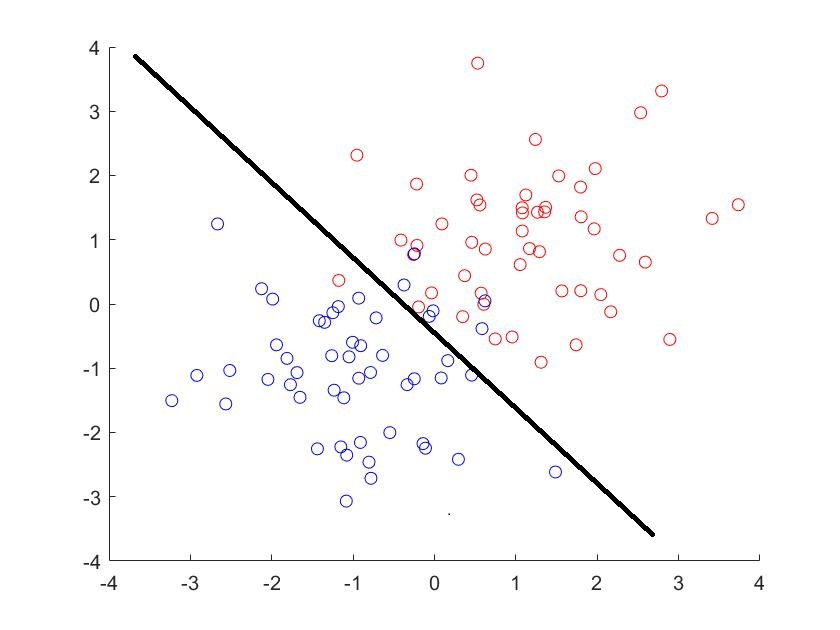
\includegraphics[width=.45\textwidth]{../Figures/2_Gaussians_with_classifier}%
	}%
	\ifdim\ht0>\ht2
	\setbox0\hbox{%
		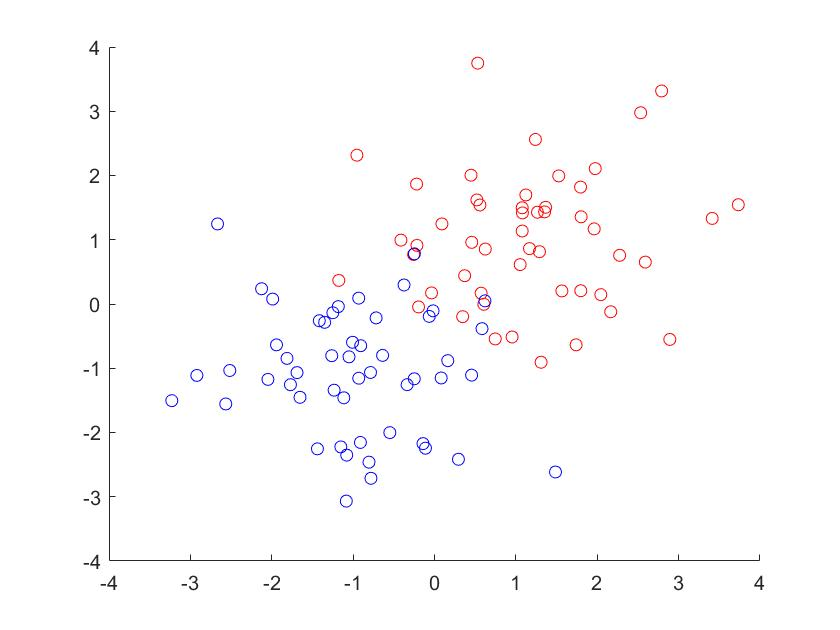
\includegraphics[height=\ht2]{../Figures/2_Gaussians}%
	}%
	\else
	\setbox2\hbox{%
		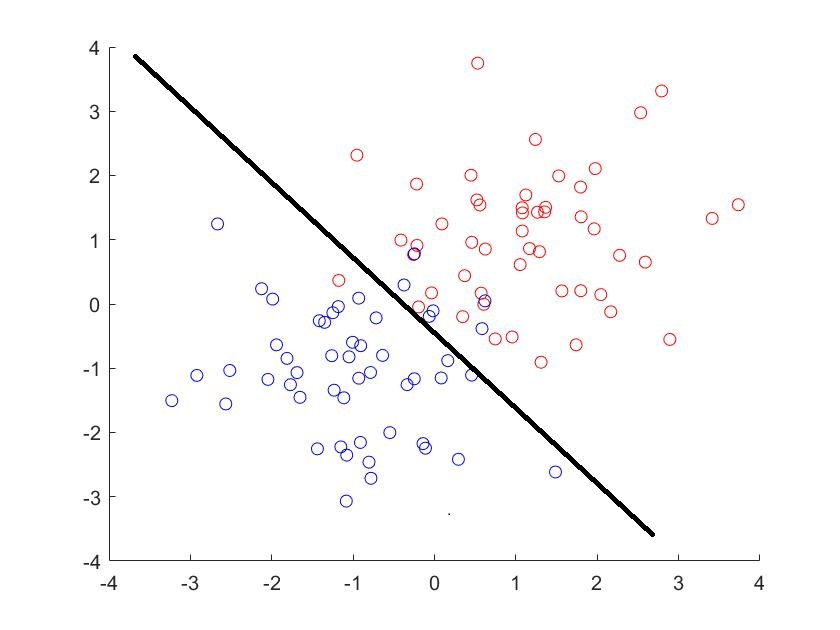
\includegraphics[height=\ht0]{../Figures/2_Gaussians_with_classifier}%
	}%
	\fi
	\noindent
	\parbox{.45\textwidth}{%
		\centering
		\unhbox0
		\caption{Two Simulated Datasets.}
	}%
	\hfil
	\parbox{.45\textwidth}{%
		\centering
		\unhbox2
		\caption{Two Simulated Datasets with Optimal Classifier.}
	}%
\end{figure}




\textbf{Given this figure, can you make a geometric construction using lines to estimate the optimal classifier? Under which conditions do you think this construction is optimal/valid?}\\

Figure 1:a is the output of the simulated datasets. As shown in figure 1:b it is possible to show an optimal classifier. This classifier is known as the Bayes Classifier. A test observation is assigned with predictor vector $x_{0}$ to the class j for which    \[ Pr(Y=j|X=x_{0}) \] is largest. The classifier is optimal because it produces the lowest possible error rate and allows for some overlap. The classifier is valid because the underlying distribution of the dataset is known. This falls into the special case $\Sigma_{xx1} = \Sigma_{xx2} - \Sigma_{xx}$, the covariance matrices are equal and the decision boundary is linear.
\subsection{The Support Vector Machine}

This section will deal with an online demo of a linear and none linear SVM. It will be used to learn the intuition behind changing SVM parameters and changes in the dataset.\\


\begin{figure}[H]
	\setbox0\hbox{%
		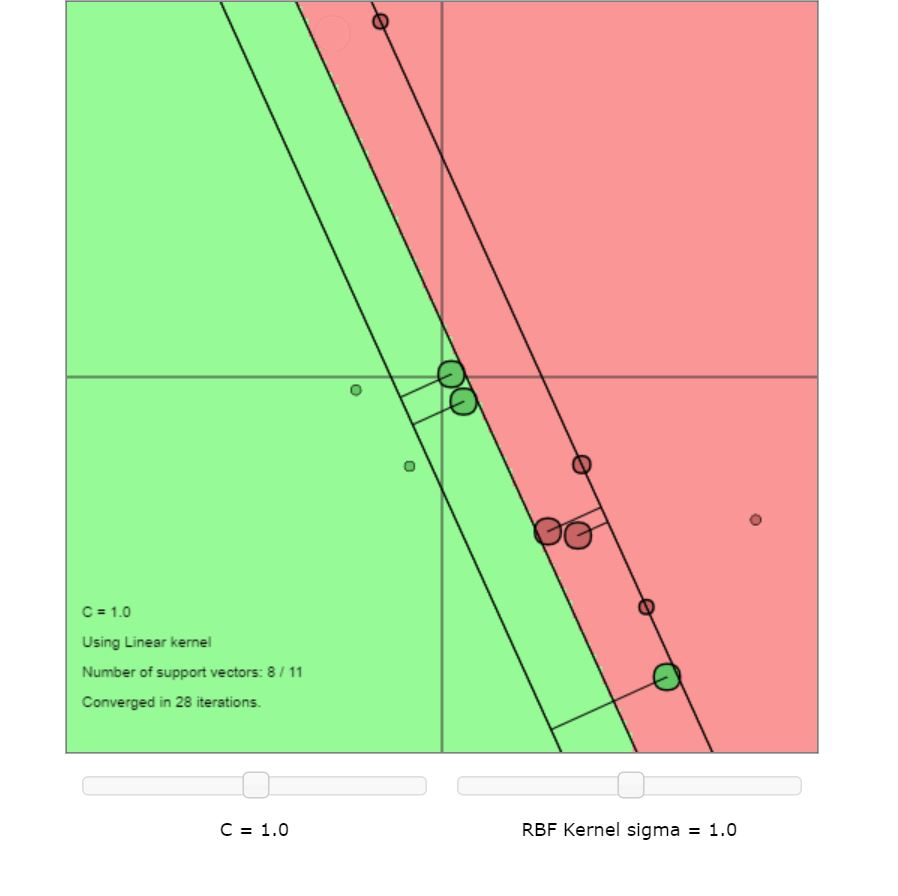
\includegraphics[width=.45\textwidth]{../Figures/Default_Linear_Kernal}%
	}%
	\setbox2\hbox{%
		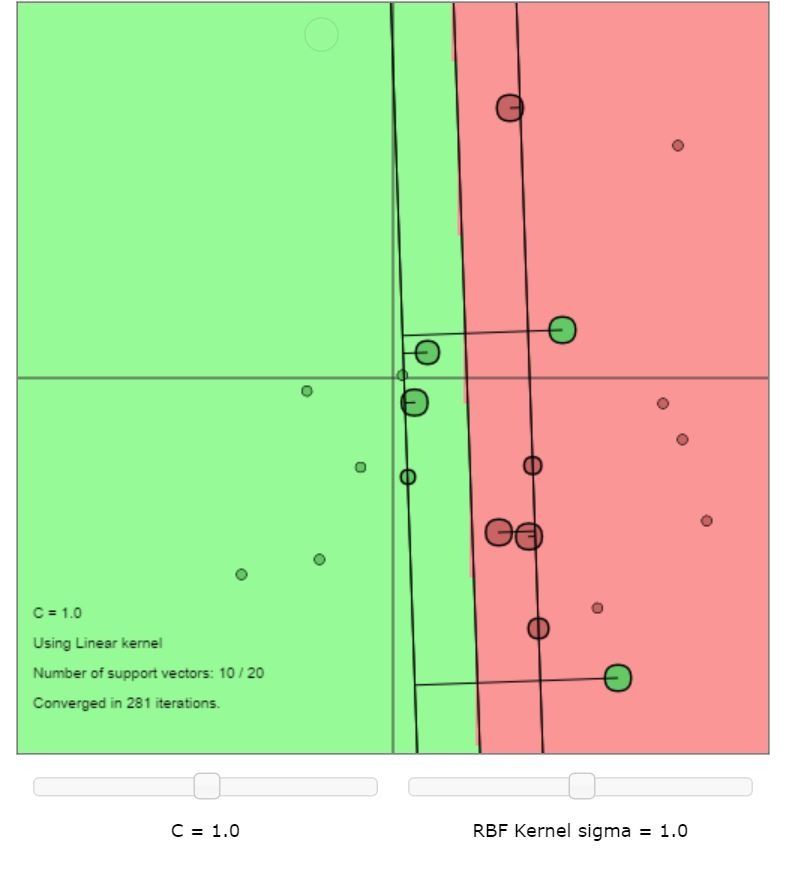
\includegraphics[width=.45\textwidth]{../Figures/10_point_linear_Kernal}%
	}%
	\ifdim\ht0>\ht2
	\setbox0\hbox{%
		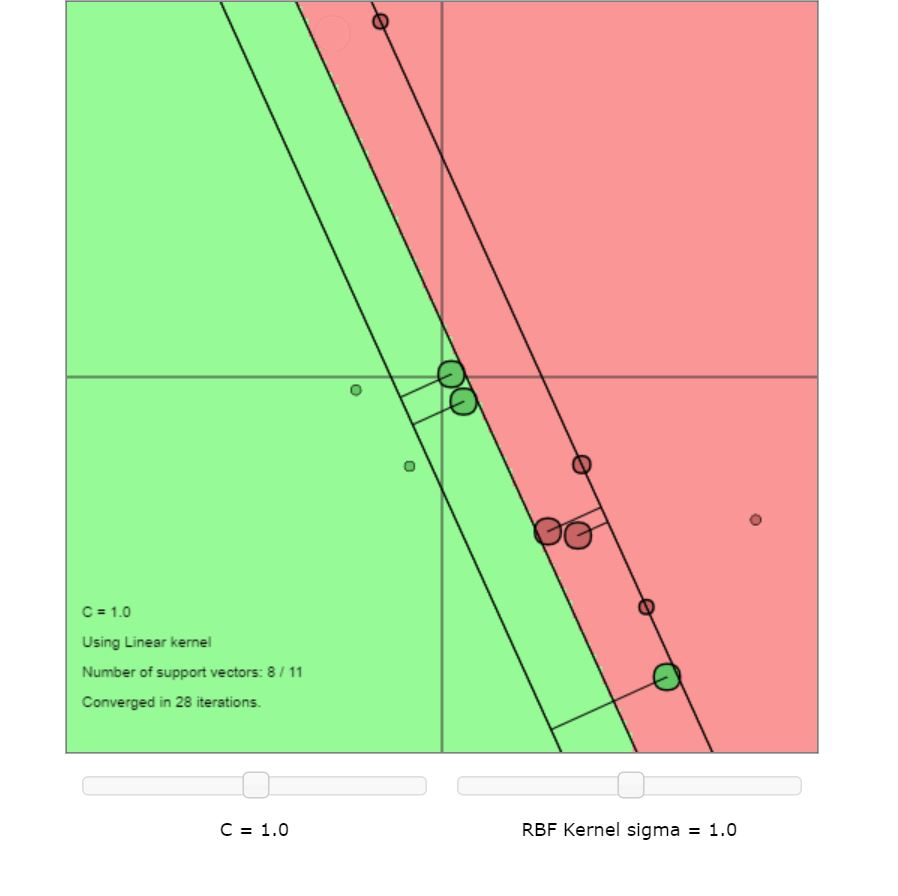
\includegraphics[height=\ht2]{../Figures/Default_Linear_Kernal}%
	}%
	\else
	\setbox2\hbox{%
		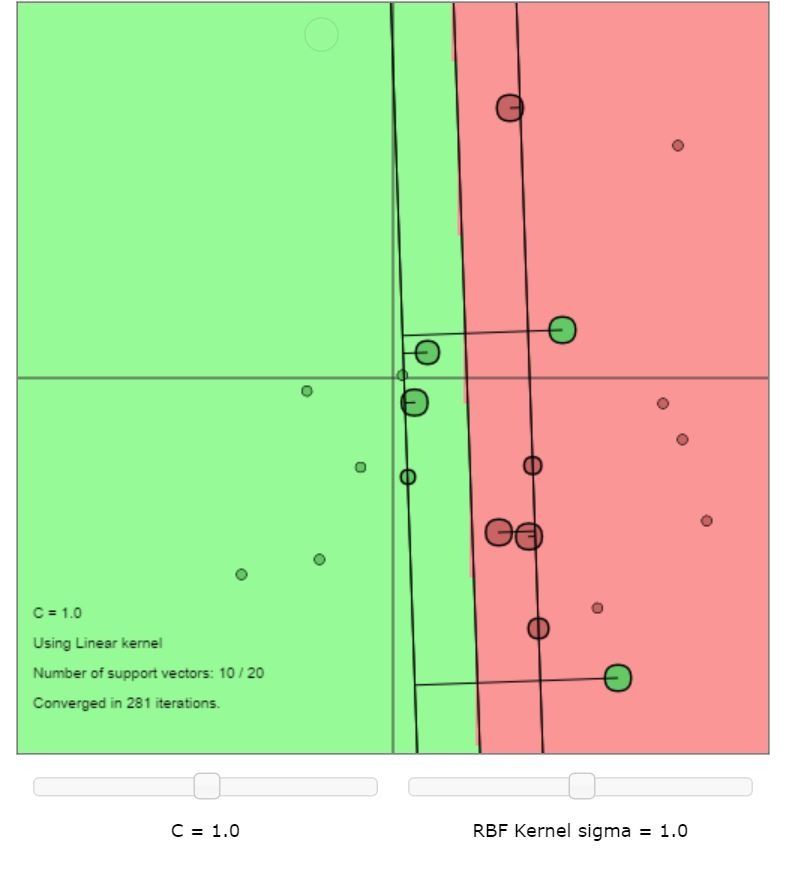
\includegraphics[height=\ht0]{../Figures/10_point_linear_Kernal}%
	}%
	\fi
	\noindent
	\parbox{.45\textwidth}{%
		\centering
		\unhbox0
		\caption{Default Linear Kernal.}
	}%
	\hfil
	\parbox{.45\textwidth}{%
		\centering
		\unhbox2
		\caption{10 Data Point Linear Kernal.}
	}%
\end{figure}

\textbf{Adjust the existing datasets to have at least 10 data points for each class. What do you observe when you are adding data points to the classes? How drastically can classification boundaries change.}

Data points added inside the margin drastically change the decision boundary  and become support vectors. Data points added to the side of the opposing color are also automatically support vectors but remain misclassified. Data points added to the same side as its own color have very little effect on the decision boundary, although the closer to the boundary the larger the effect. 

\textbf{What if you add an outlying datapoint which lies on the wrong side of the classification boundary? How does it affect the classification hyperplane?}

\begin{figure}[H]
	 \centering
	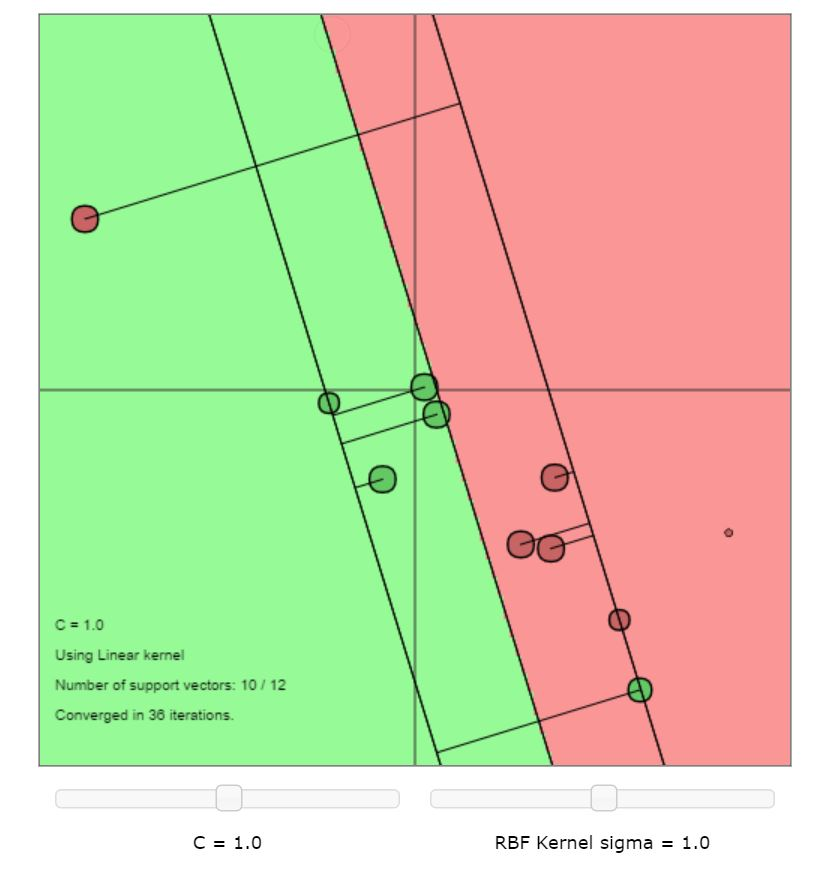
\includegraphics[scale=0.5]{../Figures/misclassified_linear_kernal}
	\caption{Outlier data point}
\end{figure}

A data point added to the wrong side of the boundary changes the direction of the hyperplane towards that point. If too many points are added the classifier misclassified all points of the opposing class. 

\textbf{Try different values of C regularization hyperparameter. How does it affect the classification outcome? What is the role of it?}\\
Using the intial dataset the effects of the regularization hyperparemter can be seen. The parameter control the slack of the SVM model. When C is high there is less tolerance for misclassification and therefore a smaller margin. When C is large there is higher tolerance for misclassification and a larger margin.

\begin{figure}[H]
	\setbox0\hbox{%
		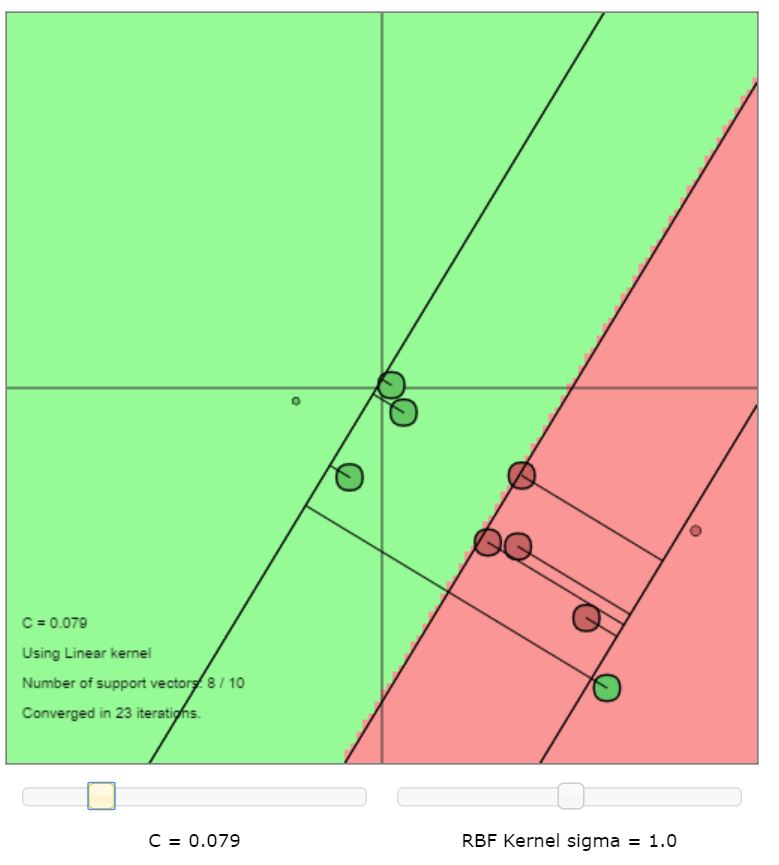
\includegraphics[width=.45\textwidth]{../Figures/small_C_linear_Kernal}%
	}%
	\setbox2\hbox{%
		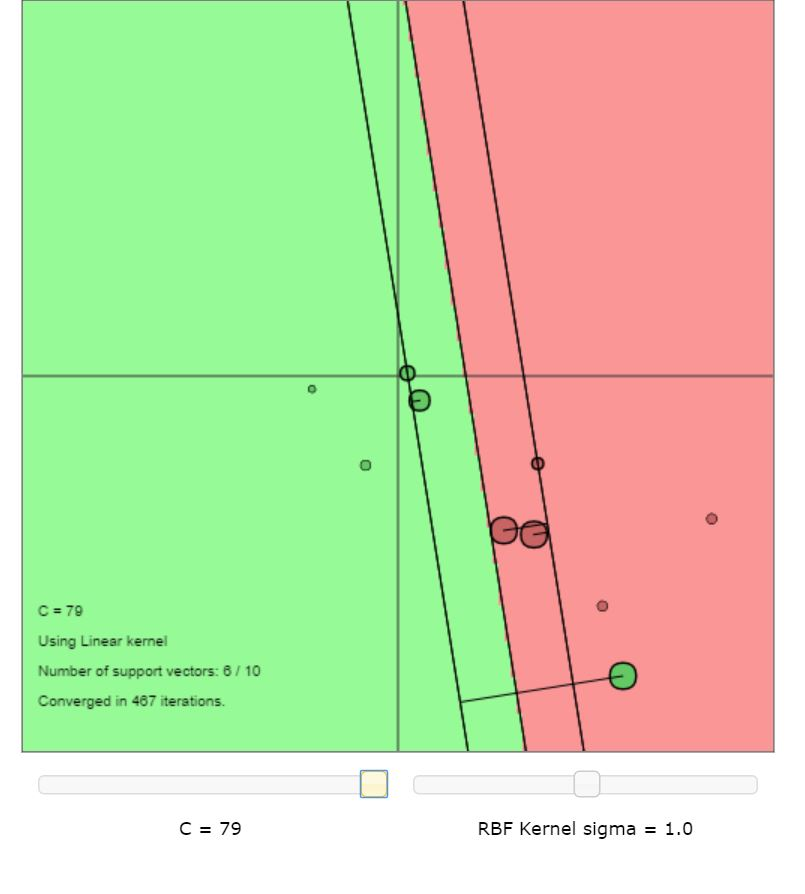
\includegraphics[width=.45\textwidth]{../Figures/large_C_linear_kernal}%
	}%
	\ifdim\ht0>\ht2
	\setbox0\hbox{%
		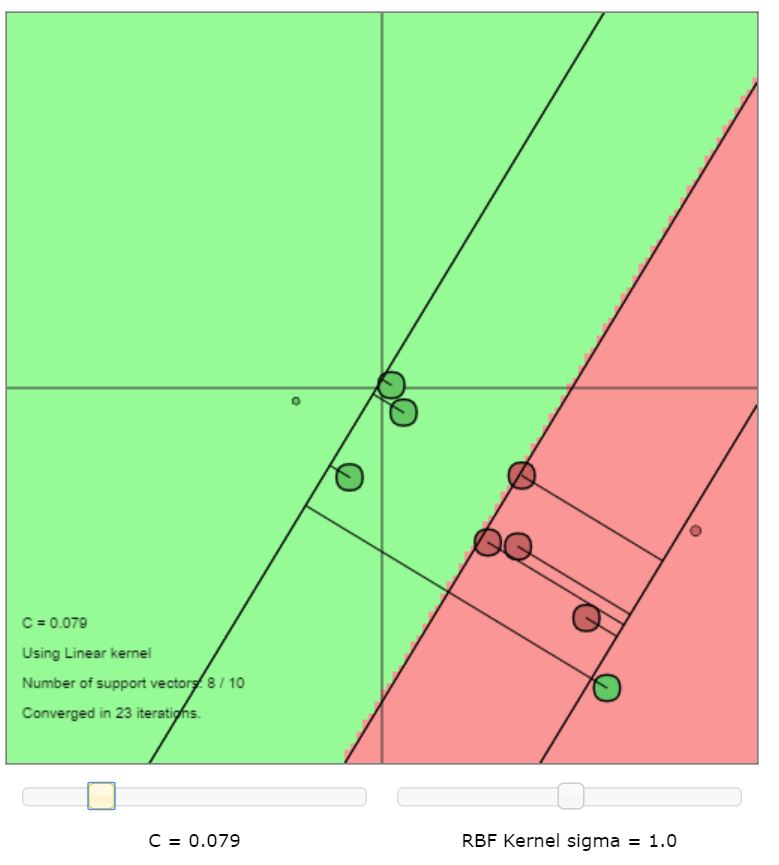
\includegraphics[height= \ht2]{../Figures/small_C_linear_Kernal}%
	}%
	\else
	\setbox2\hbox{%
		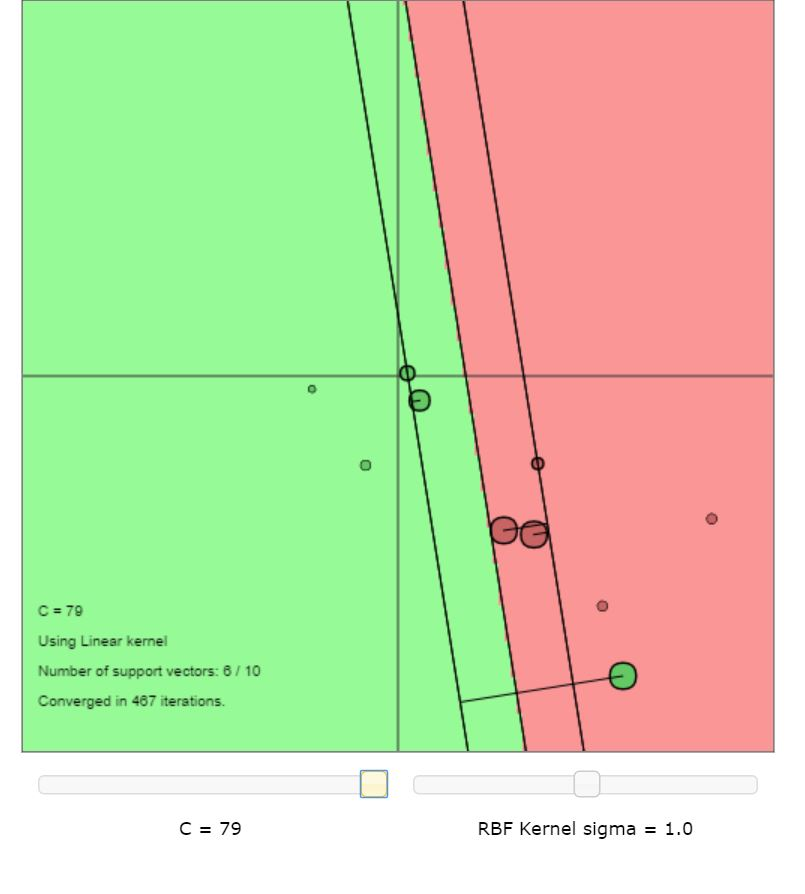
\includegraphics[height=\ht0]{../Figures/large_C_linear_kernal}%
	}%
	\fi
	\noindent
	\parbox{.45\textwidth}{%
		\centering
		\unhbox0
		\caption{C = .079}
		\label{fg:methods}
	}%
	\hfil
	\parbox{.45\textwidth}{%
		\centering
		\unhbox2
		\caption{C = 79}
		\label{fg:method_detail}
	}%
\end{figure}

 

 \begin{figure}[H]
 	\centering
 	\begin{subfigure}[b]{.5\textwidth}
 	
 		\textbf{Follow the instructions and switch back to RBF kernel by toggling the “k” button. Compare to the classification outcome of the linear case.Try to change the RBF kernel sigma hyper parameter. What is your intuition? How does it affect the classification boundaries? Now try to change both hyper parameters. What is the right choice of those if your data is almost linearly separable?}\\
 		
		 The default RBF kernal has no misclassification as opposed to the linear classifier. This is because the data set is not linearly separable, therefore the linear classifier performs poorly. The RBF kernal has the ability to wrap around the data. Small values of  $\sigma$ however will lead to a risk of over fitting and generalize well. Misclassification is only seen at the higher end of  $\sigma$. The higher  $\sigma$  is the more linear the decision boundary. \\
		 
		 The right choice to make when the data is almost linear separable is the linear kernel. As stated above, data that is almost linearly separable but has some overlap can be best classified using Bayes Optimal classifier. This will lead to a linear decision boundary with some misclassification. If an RBF kernel is chosen you may have good predictions on your validation data but the model will not generalize to the test data. Using the RBF kernal you can get a near linear decision boundary with $ c = 79$ and $\sigma = 10$
		 
 		
 	
 	\end{subfigure}%
 	\begin{subfigure}{.5\textwidth}
 		\vspace{-185pt}
 		\centering
 		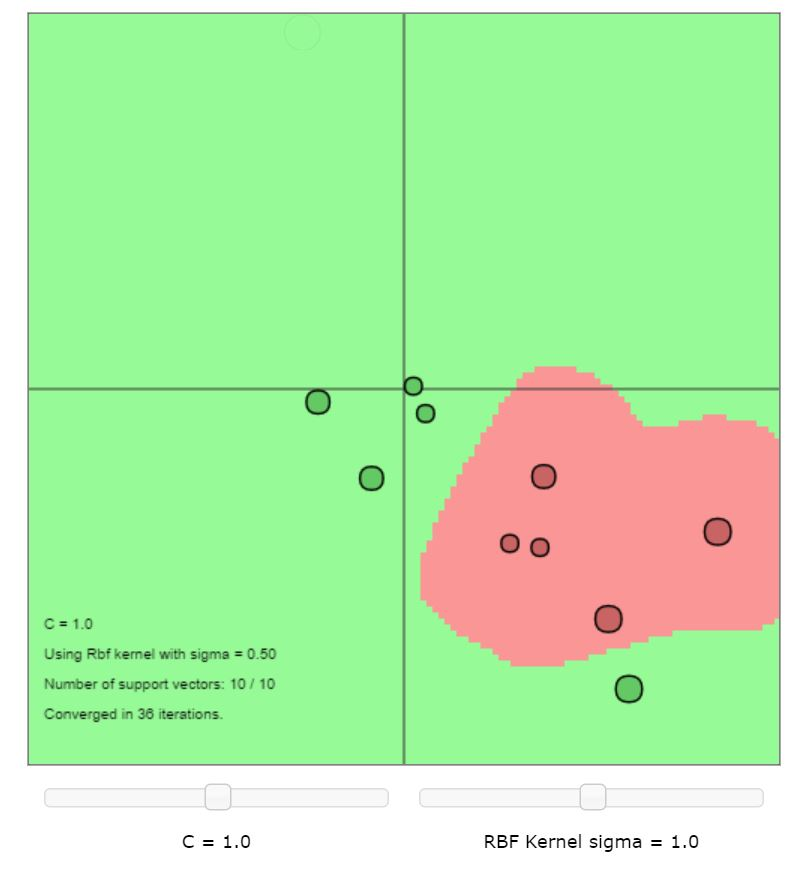
\includegraphics[width=0.9\linewidth]{../Figures/Default_RBF}
 	\end{subfigure}
 \end{figure}
\begin{figure}[H]
	\centering
 		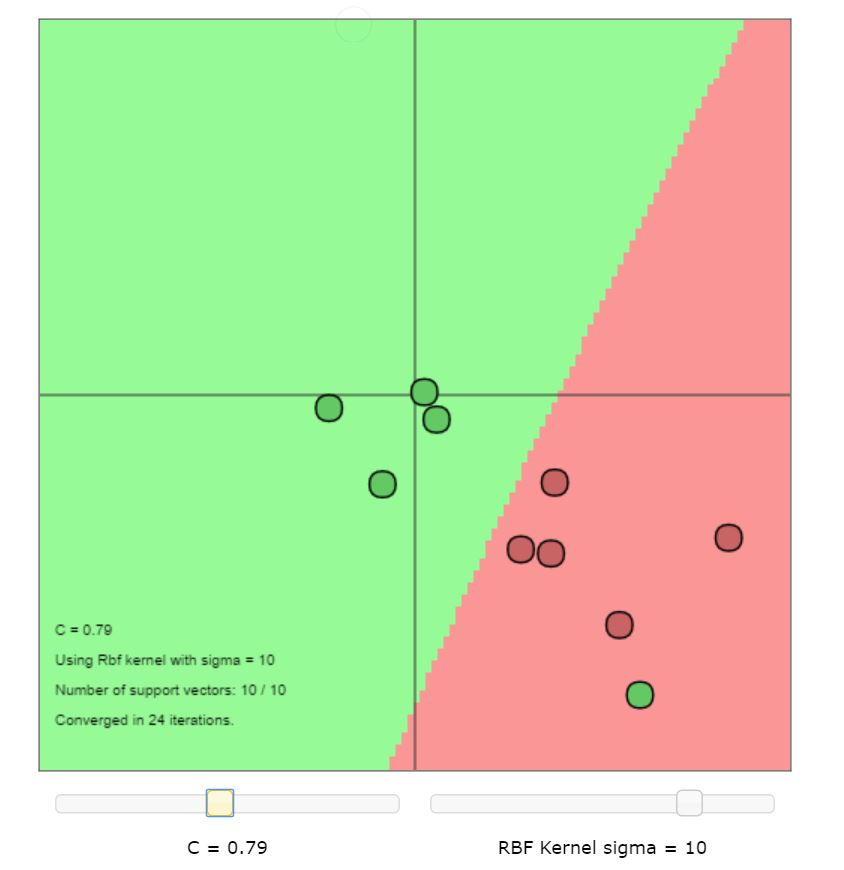
\includegraphics[scale=0.5]{../Figures/RBF_sigma_10_C_079}
 		\caption{Value of $\sigma = 0.79$}
\end{figure}
 \begin{figure}[H]
 	\centering
 	\begin{subfigure}{.25\textwidth}
 		\centering
 		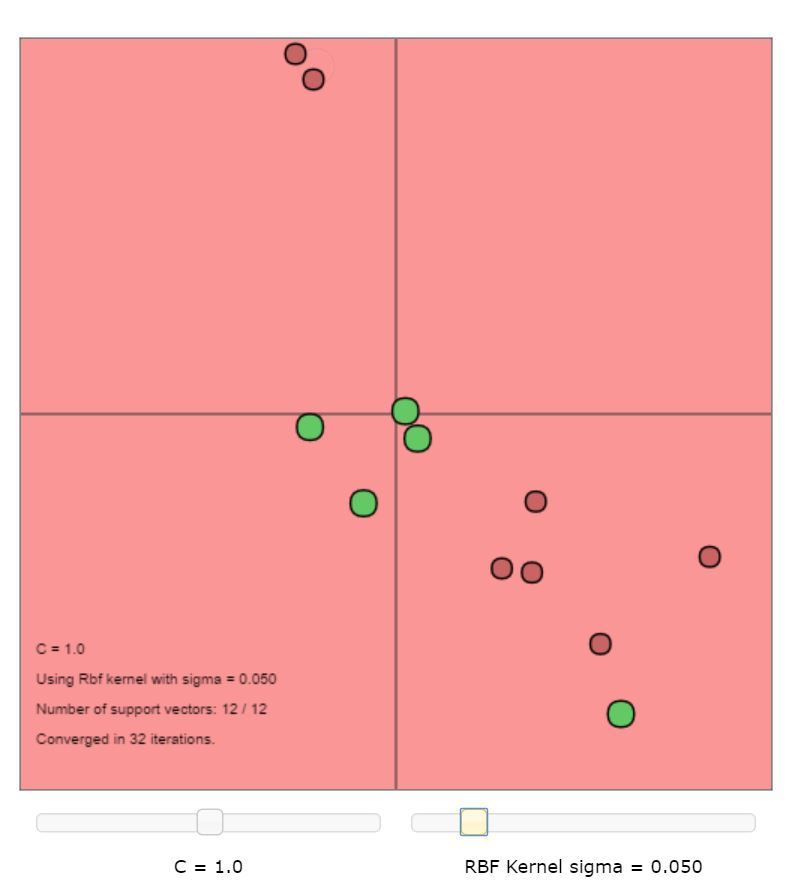
\includegraphics[width=0.9\linewidth]{../Figures/RBF_sigma_0050}
 		\caption{Value of $\sigma = 0.050$}
 	\end{subfigure}%
 	\begin{subfigure}{.25\textwidth}
 		\centering
 		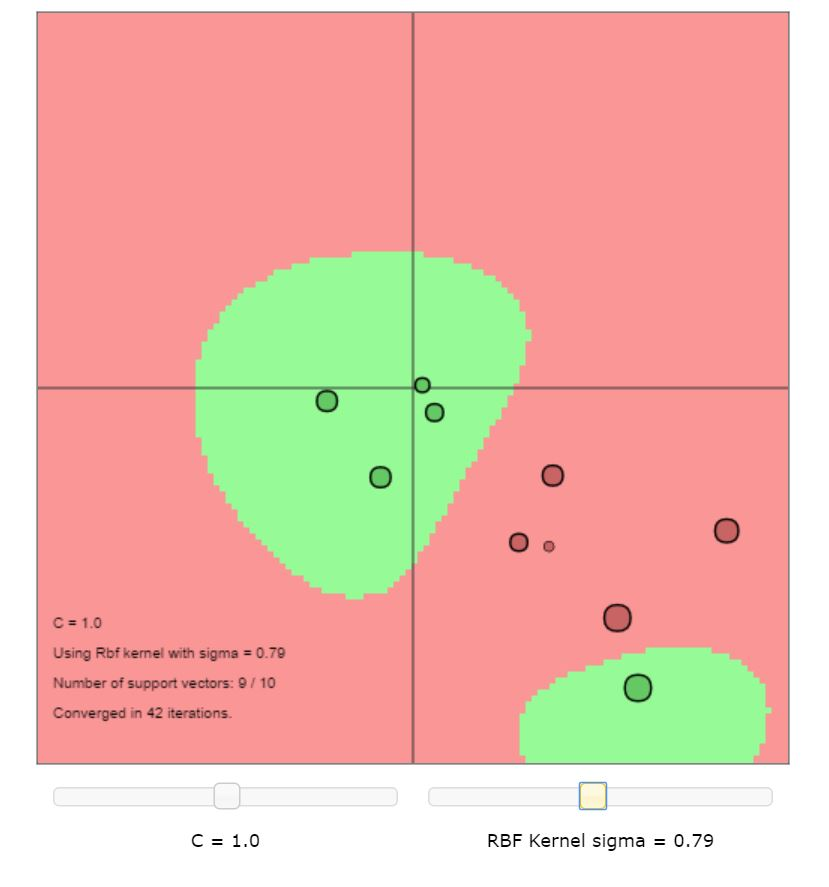
\includegraphics[width=0.9\linewidth]{../Figures/RBF_sigma_79}
 		\caption{Value of $\sigma = 0.79$}
 	\end{subfigure}%
 	\begin{subfigure}{.25\textwidth}
 		\centering
 		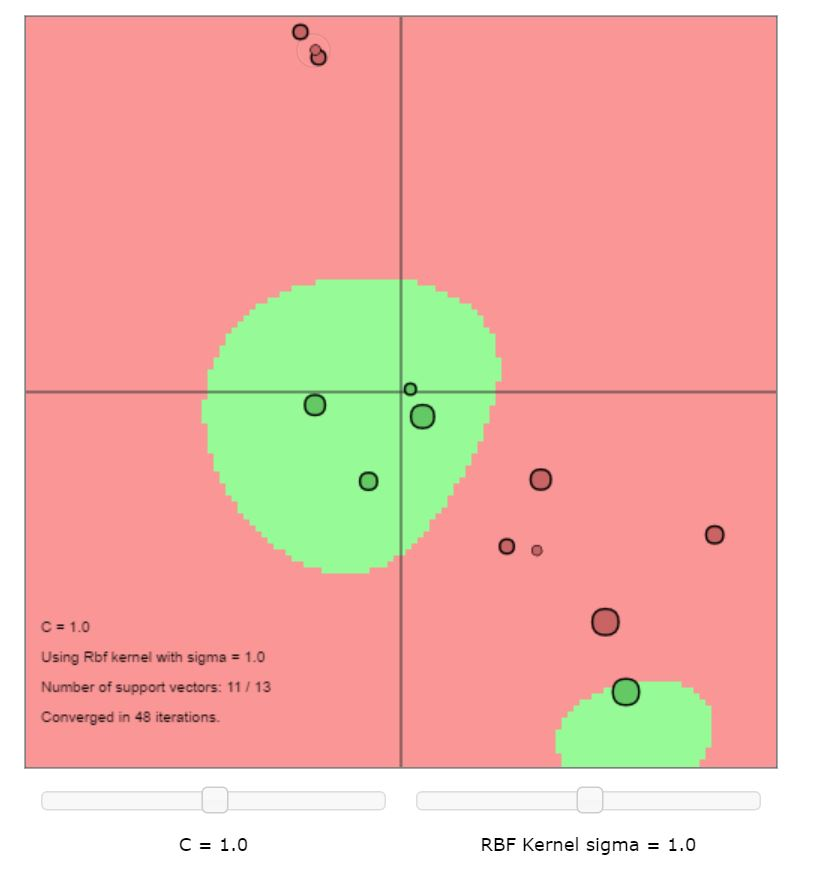
\includegraphics[width=0.9\linewidth]{../Figures/RBF_sigma_1}
 		\caption{Value of $\sigma = 1$}
 	\end{subfigure}%
 	\begin{subfigure}{.25\textwidth}
 		\centering
		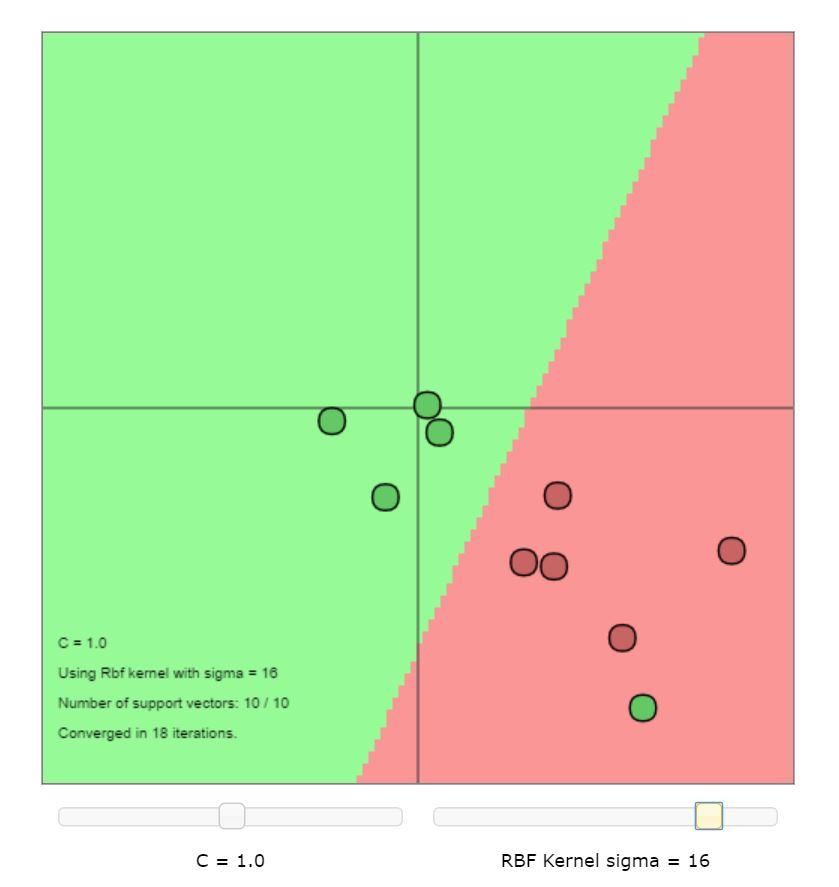
\includegraphics[width=0.9\linewidth]{../Figures/RBF_sigma_16}
 		\caption{Value of $\sigma = 16$}
 	\end{subfigure}
 	\caption{How $\sigma$ effects RBF classifier with C = 1.0}
 \end{figure}
 
 \begin{figure}[H]
 	\centering
 	\begin{subfigure}[b]{.5\textwidth}
 		
 	\textbf{Create a linearly non-separable dataset with an overlapping region between classes (e.g. similar to the previous Gaussian clouds). Give comments on the role of the chosen kernel, the regularization parameter (C) and the kernel parameter (sigma)}\\
 	
 		For this set 25 red and 25 green points were created. These points were made to create a dataset as described above. An RBF kernel was chosen because the dataset is not linearly separable so using a linear kernel would be impossible. The parameters were chosen to appropriately classify the data points but also to leave some slack for misclassification. Due to the overlapping regions, if everything was perfectly classified on this validation set you would most likely see an over fitting when you introduce your test set. The C and sigma values were adjusted accordingly. The C value was chosen relatively high to allow for the misclassification. The Sigma is relatively small because a large sigma would cause a near linear decision boundary which would be useless in this case. 
 		
 		
 		
 	\end{subfigure}%
 	\begin{subfigure}{.5\textwidth}
 		\vspace{-185pt}
 		\centering
 		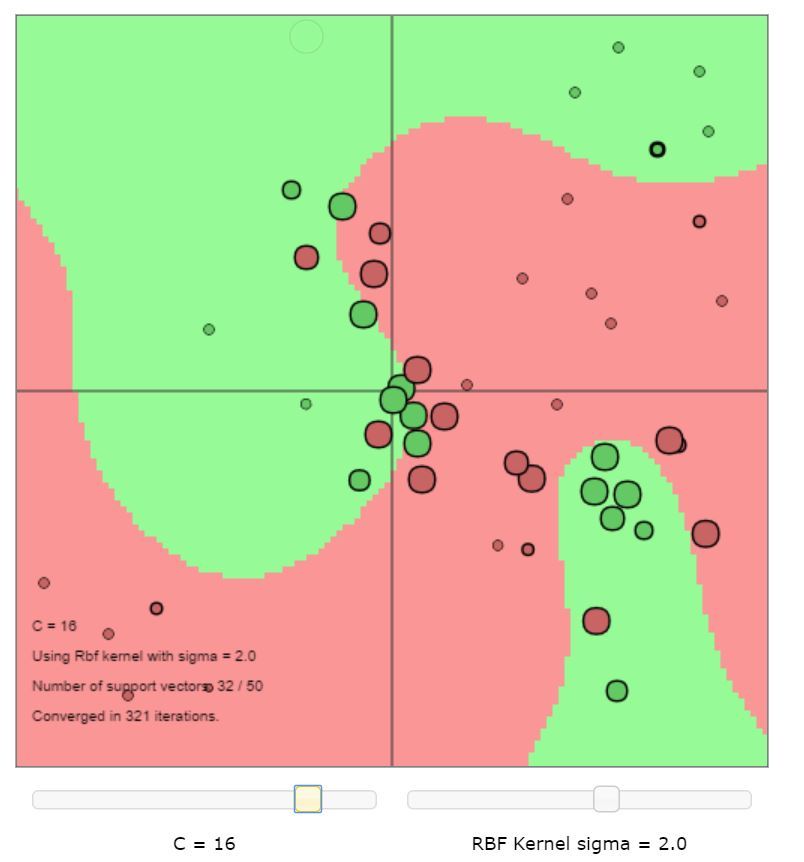
\includegraphics[width=0.9\linewidth]{../Figures/RBF_non_linear_data}
 	\end{subfigure}
 \end{figure}

\textbf{What is the role of Support Vectors? Change the data-sets to make the number of support vectors
increase/decrease. When does a particular datapoint become a Support Vector?}\\
	As a property of this being a quadratic programming problem that is  a dual problem many resulting values of $ \alpha_{k}$ are equal to zero in the classifier $ y(x)= sign[\sum_{k = 1}^{\#SV} \alpha_{k} y_{k} x_{k}^{T}x + b] $ This is a property called sparseness. The sum is of the none zero $\alpha_{k}$ which are now support vectors. Geometrically they are located close to the decision boundary. In a linear kernel all vectors inside or at the edge of the margin are support vectors as well as misclassified data points. For the RBF kernel $x$ is replaced by $\varphi(x)$. However this can be infinite dimensional. Therefore the problem can only be solved in the dual. 
	
\textbf{When does the corresponding importance of a Support Vector change?}\\
The importance of support vector changes when the influence it has on the decision boundary is altered. This can happen when changing the c parameter.

\subsection{Using LSSVM}
In this section the matlab package LSSVM will be used to explore the Iris Dataset.

\begin{figure}[H]
	\centering
	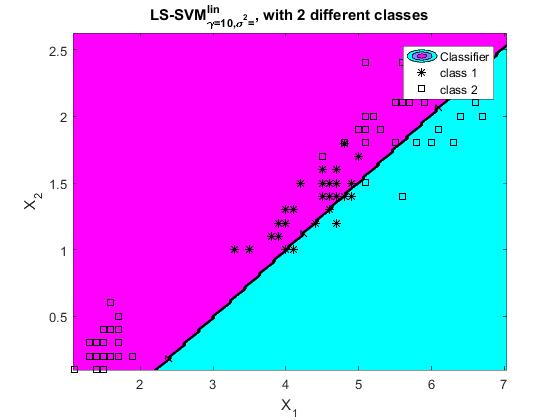
\includegraphics[scale=0.5]{../Figures/iris_intial}
	\caption{Value of $\sigma = 0.79$}
\end{figure}

\textbf{What is the performance on the test set Xt and Yt?}\\
The performance shows a $55\%$ error rate.

\textbf{What happens when you are changing the degree of a polynomial kernel? Explain the obtained results.
Does it correspond to the changes in sigma hyperparameter of the RBF kernel in the previous example?}\\\

The first degree polynomial is just a linear kernel, therefore it has the same results. The 2nd degree has 4 misclassification. The 3rd degree has 3 misclassification. The 4th degree has 3 and the 5th has 3. Increasing the degree of polynomial is a little like decreasing sigma of the RBF. It creates a less linear boundary that is more prone to over fitting. 

\begin{figure}[H]
	\begin{subfigure}[b]{0.4\textwidth}
		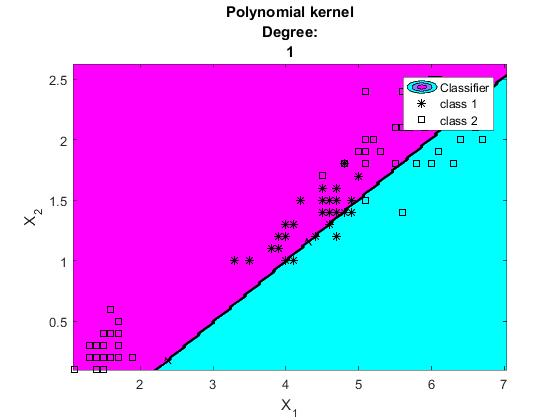
\includegraphics[width=\textwidth]{../Figures/poly_degree_1}
		\caption{Degree 1}
	\end{subfigure}
	%
	\begin{subfigure}[b]{0.4\textwidth}
		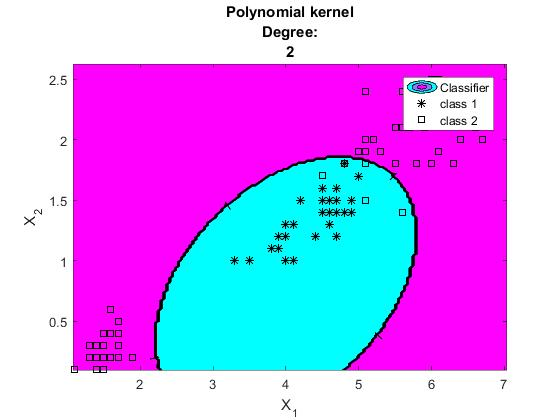
\includegraphics[width=\textwidth]{../Figures/poly_degree_2}
		\caption{Degree 2}
	\end{subfigure}
	%
	\begin{subfigure}[b]{0.4\textwidth}
		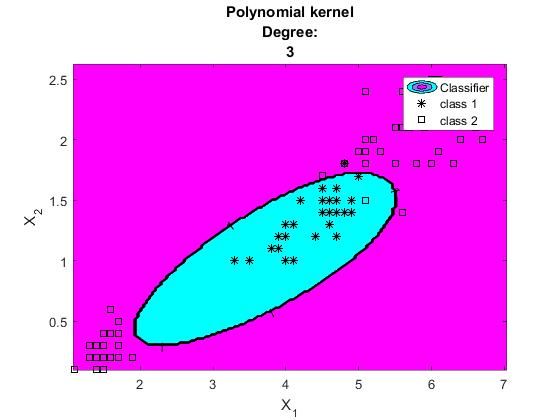
\includegraphics[width=\textwidth]{../Figures/poly_degree_3}
		\caption{Degree 3}
	\end{subfigure}
	%
	\begin{subfigure}[b]{0.4\textwidth}
		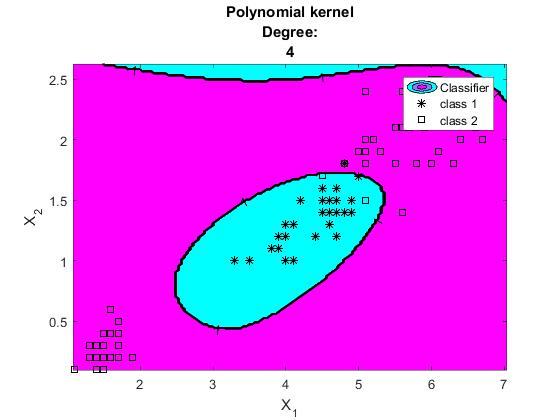
\includegraphics[width=\textwidth]{../Figures/poly_degree_4}
		\caption{Degree 4}
	\end{subfigure}
	%
	\begin{subfigure}[b]{0.4\textwidth}
	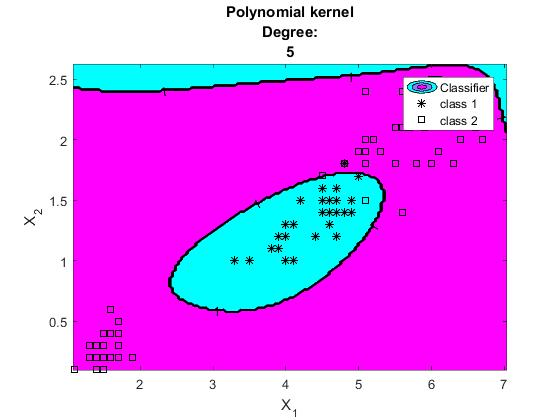
\includegraphics[width=\textwidth]{../Figures/poly_degree_5}
	\caption{Degree 5}
\end{subfigure}
\caption{Varying Degrees of the Polynomial Kernel}
\end{figure}
\textbf{Try out a good range of
different sig2’s as kernel parameters. For each individual value of sig2, the corresponding LS-SVM
is evaluated on the test set. Make a figure of the sig2’s with their corresponding test set performance. Fix a reasonable choice for the sig2 of the RBF
kernel and again compare a range of gam’s by plotting the corresponding test set performances. What
is a good range for gam?}\\
\begin{figure}[H]
	\centering
	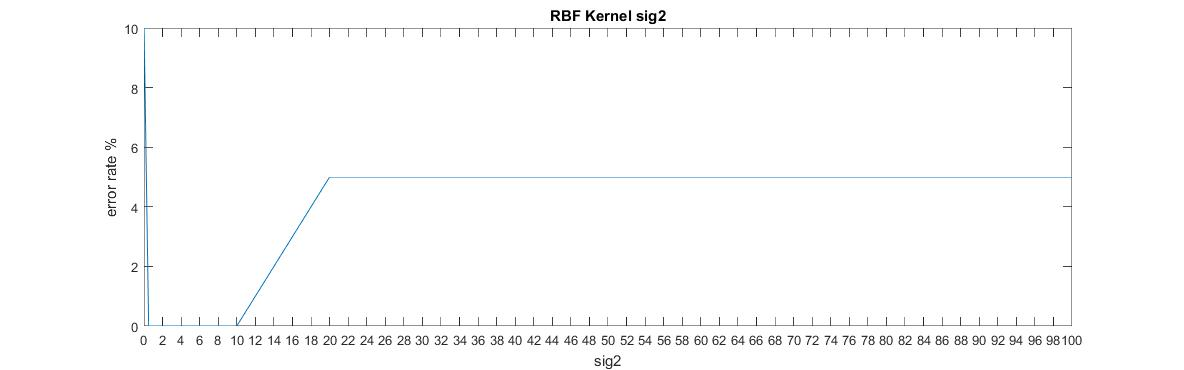
\includegraphics[scale=0.4]{../Figures/RBF_sig2}
	\caption{Error rate VS. Sig2}
\end{figure}
A range used for both sig2 and gamma was 0.01, 0.5, 4, 10, 20, 100.Between point 5 and 14 seem to have the best range for sig2. With a sig2 of 12 the best gam is between 2 and 8.   
\begin{figure}[H]
	\centering
	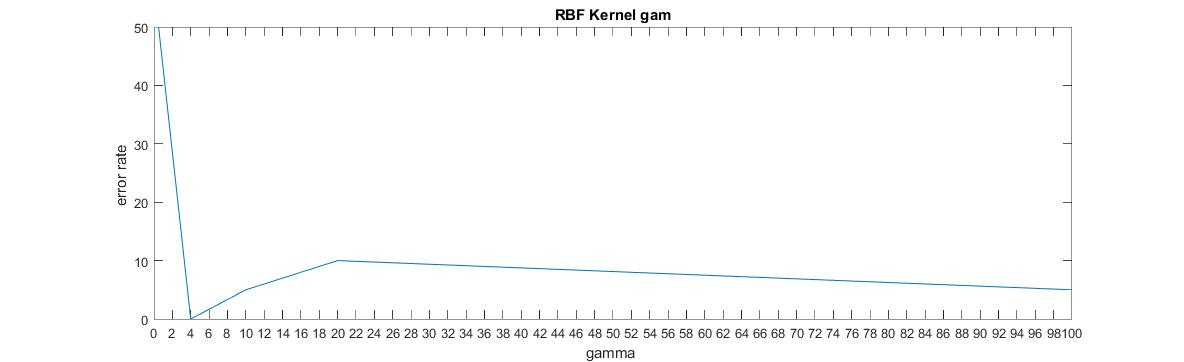
\includegraphics[scale=0.4]{../Figures/RBF_gam}
	\caption{Error rate VS. gam}
\end{figure}

Comparing to the results from the sample script you get a very similar outlook. You need a good balance between gam and sig to balance between over fitting and misclassification. 

\subsection{Choice of Hyper-parameters}
In this section the intuition developed from the previous sections will be used to start using autotuning algorithms. \\

\textbf{Motivate why this validation set used to optimize a number of(tuning-) parameters cannot used again to measure the final model.} \\

Validation set is used to optimize parameters to make sure that the model can generalize well. If someone was to just train the model on one data set and validate it on another without using a test set the model will likely "memorize the data" (difference between 'dumb' AI and smart 'AI'). Therefore a set of data that was not touched during the tuning process must be the final test to see if the model can generalize. 

\begin{figure}[H]
	\begin{subfigure}[b]{0.5\textwidth}
		\includegraphics[width=\textwidth]{../Figures/valerrorg}
		\caption{Error for Gam values 1, 10, 100 with sig2 = 1}
	\end{subfigure}
	%
	\begin{subfigure}[b]{0.5\textwidth}
		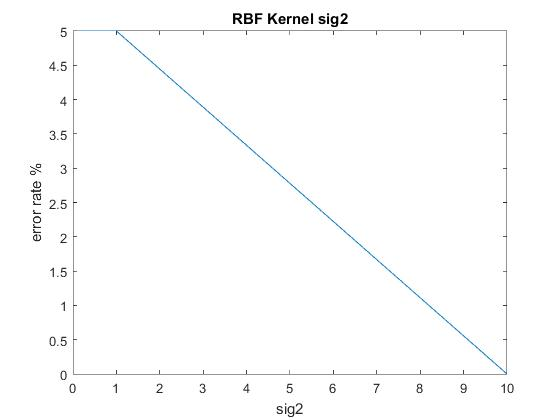
\includegraphics[width=\textwidth]{../Figures/Valerror}
		\caption{Error for Sig values 0.1,1,10 with gam = 10}
	\end{subfigure}
	\caption{Tuning}
\end{figure}

Across the different values the error does not really change. It stays steady across all values of gam and sig2 except for when cig2 is 10, then you see a 50\% decrease in error.

\textbf{Think about a clear and intuitive way to represent this technique. Why should one prefer this method
over a simple validation? Change crossvalidate procedure for leaveoneout (removing the
10). Is it giving better results? In which cases one would prefer each?}\\

They both perform exactly the same. Leave one out would be prefered when the data set is very large. Leave one out is computationally expensive. LOOCV also gives you a hire chance of over fitting since your model has seen all of your data. 

\textbf{Try to change different parameters like 'csa' (Coupled Simulated Annealing) vs. 'ds' (Randomized
Directional Search) and 'simplex' (Nelder-Mead method) vs. 'gridsearch' (brute force
gridsearch). What differences do you observe? Why in some cases the obtained hyperparameters differ
a lot?}\\

Since there is an element of randomness each run will yield different results. Since this is finding hyper parameters the problem in non-convex and local minima can occur. 

The ROC is often used to asses a model. It is important not to use this on the validation set. It is for the same reason you do not judge a model based on the validation set. Models that memorize their data are not good models. Models must generalize well. 

\begin{figure}[H]
	\centering
	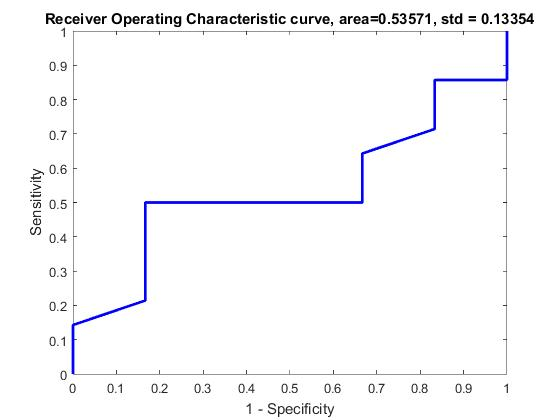
\includegraphics[scale=0.4]{../Figures/ROC}
	\caption{Error rate VS. gam}
\end{figure}

\subsection{Playing around with data}

This section will be about apply techniques learned in a more tutorial based setting to real date sets. A set of 5 questions will be answered about each data set.

\subsubsection{Ripley Dataset}


\textbf{1. Look at the plotted data. What seems to be important properties of the data?}\\

The data is split into four distinct groups with slight over lap. 
\begin{figure}[H]
	\centering
	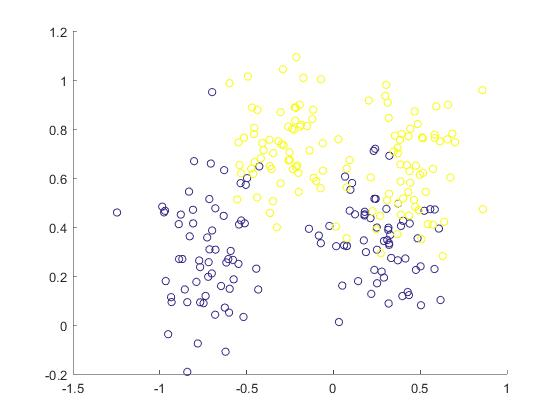
\includegraphics[scale=0.4]{../Figures/ripley_vis}
	\caption{data visualized}
\end{figure}

\textbf{2. Try a linear model. Do you think it’s sufficient?}\\
The linear model cannot model this data at all. This is because the data is not linearly separable. 

\begin{figure}[H]
	\centering
	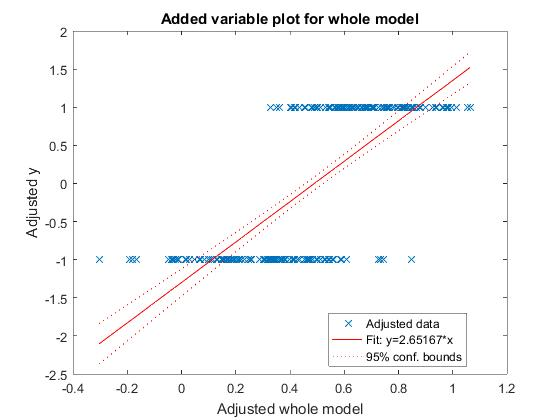
\includegraphics[scale=0.4]{../Figures/ripley_linear}
	\caption{Linear Model for ripley }
\end{figure}

\textbf{3. Try the RBF kernel and tune its parameter. Is the tuning acceptable? Run several times the routine tunelssvm. Do the tuned parameters gam and sig2 change? What about the performance?}\\

\begin{figure}[H]
	\begin{subfigure}[b]{0.4\textwidth}
		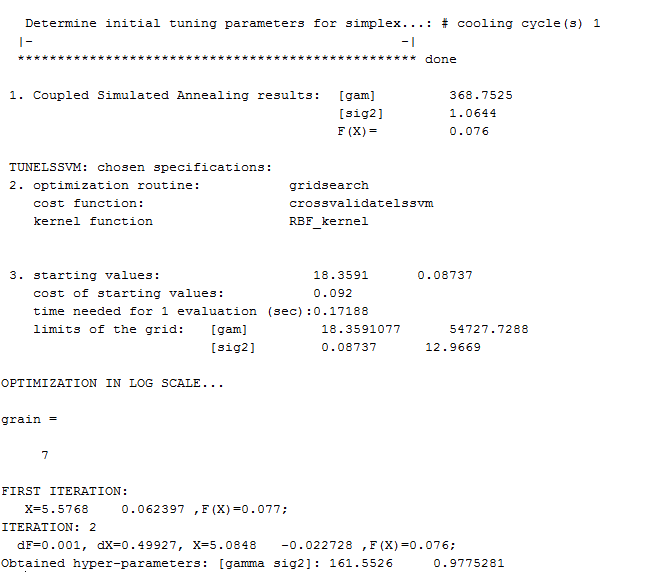
\includegraphics[width=\textwidth]{../Figures/ripley_CSA_grid}
		\caption{CSA and gridsearch}
	\end{subfigure}
	%
	\begin{subfigure}[b]{0.4\textwidth}
		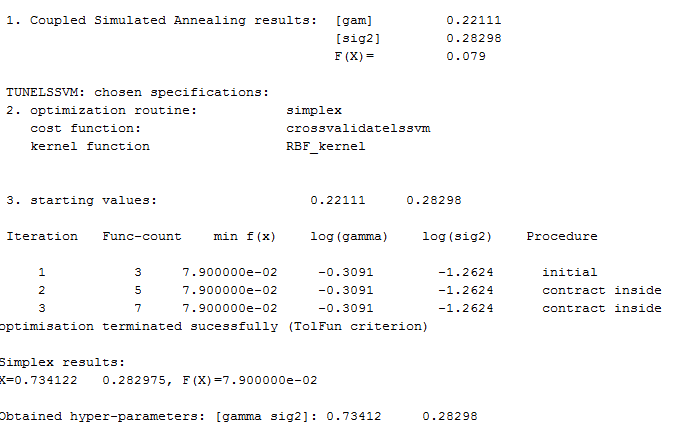
\includegraphics[width=\textwidth]{../Figures/ripley_CSA_simp}
		\caption{CSA and simplex}
	\end{subfigure}
	%
	\begin{subfigure}[b]{0.4\textwidth}
		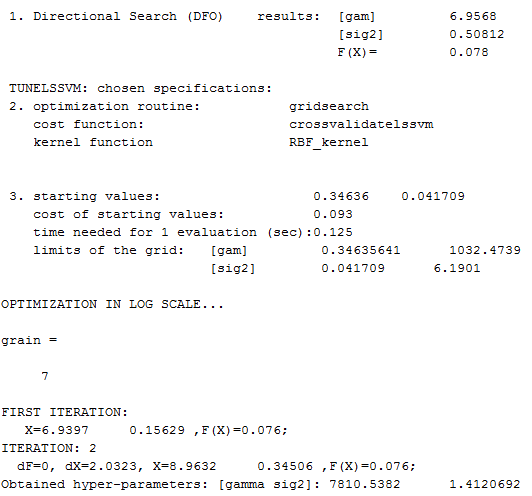
\includegraphics[width=\textwidth]{../Figures/ripley_DS_grid}
		\caption{DS and grid search}
	\end{subfigure}
	%
	\begin{subfigure}[b]{0.4\textwidth}
		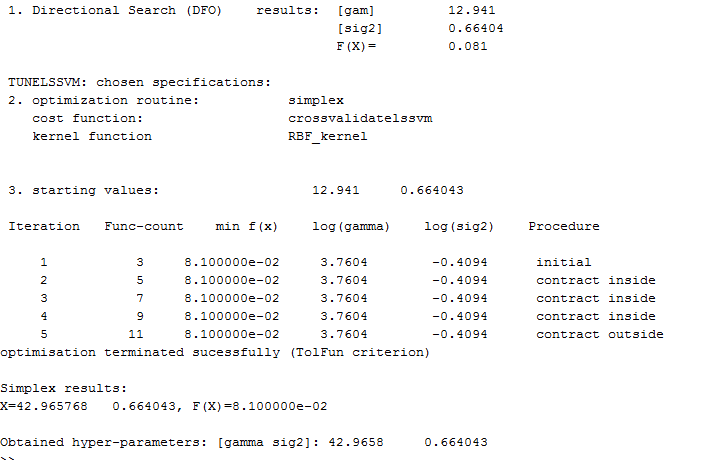
\includegraphics[width=\textwidth]{../Figures/ripley_DS_simp}
		\caption{DS and simplex}
	\end{subfigure}
	\caption{Different tuning methods}
	
\end{figure}

\textbf{5. Judge your final model. Is the methodology perfectly suited for this data-set?}
It is well suited but with such a high AUC it may be prone to overfitting.

\subsubsection{Diabetes Dataset}

\textbf{1. Look at the plotted data. What seems to be important properties of the data?}\\

This data is almost completely indistinguishable from each other. There is almost complete overlap between the two data sets. 
\begin{figure}[H]
	\centering
	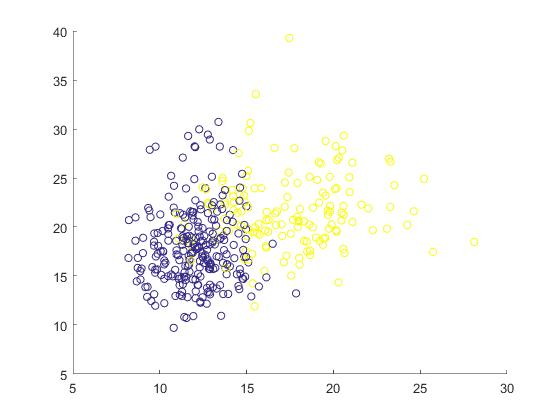
\includegraphics[scale=0.4]{../Figures/breast_viz}
	\caption{Data viz for breast }
\end{figure}

\textbf{2. Try a linear model. Do you think it’s sufficient?}\\

\begin{figure}[H]
	\centering
	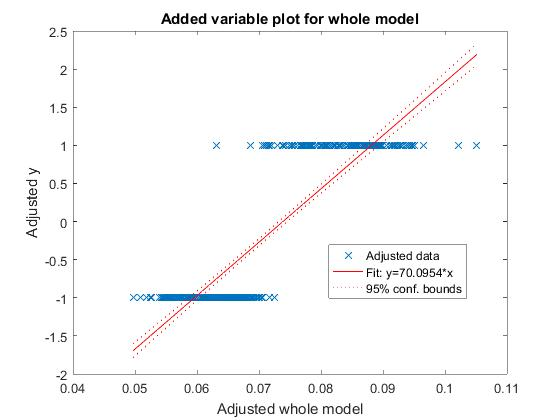
\includegraphics[scale=0.4]{../Figures/breast_lin}
	\caption{Linear Model for  breast }
\end{figure}

The linear model is not sufficient.\\
\textbf{3. Try the RBF kernel and tune its parameter. Is the tuning acceptable? Run several times the routine tunelssvm. Do the tuned parameters gam and sig2 change? What about the performance?}\\


\begin{figure}[H]
	\begin{subfigure}[b]{0.4\textwidth}
		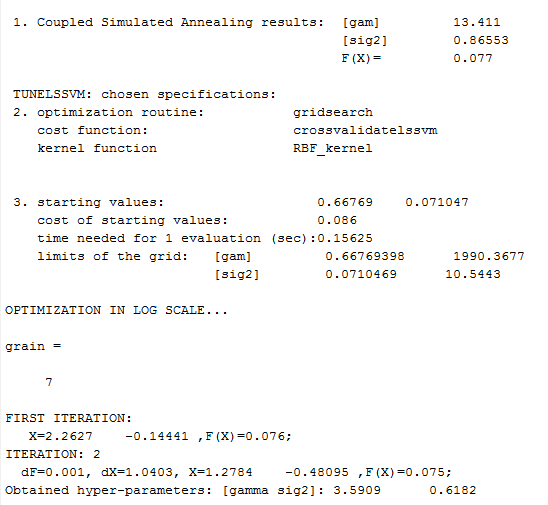
\includegraphics[width=\textwidth]{../Figures/breast_CSA_grid}
		\caption{CSA and gridsearch}
	\end{subfigure}
	%
	\begin{subfigure}[b]{0.4\textwidth}
		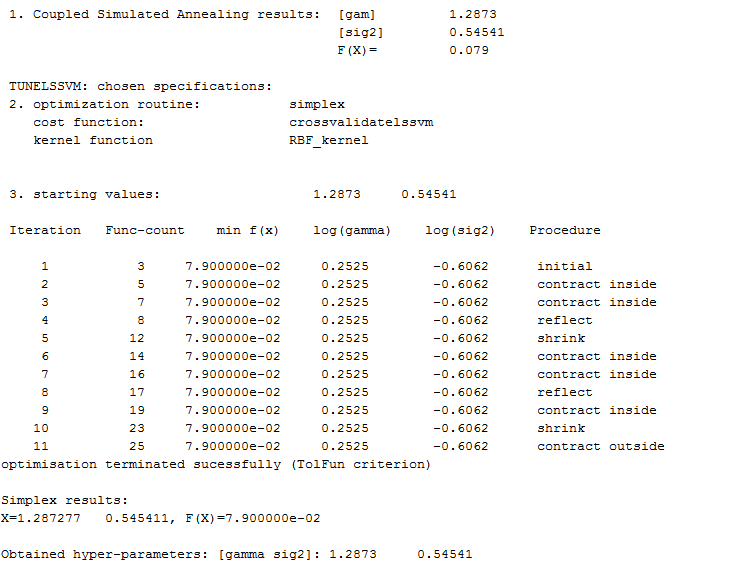
\includegraphics[width=\textwidth]{../Figures/breast_CSA_simp}
		\caption{CSA and simplex}
	\end{subfigure}
	%
	\begin{subfigure}[b]{0.4\textwidth}
		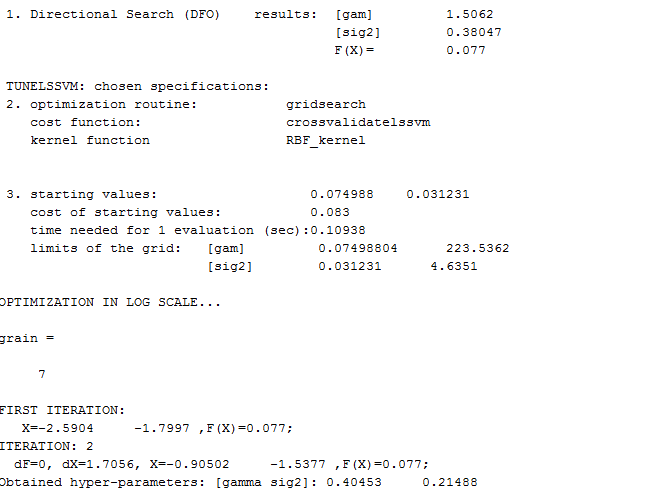
\includegraphics[width=\textwidth]{../Figures/breast_DS_grid}
		\caption{DS and grid search}
	\end{subfigure}
	%
	\begin{subfigure}[b]{0.4\textwidth}
		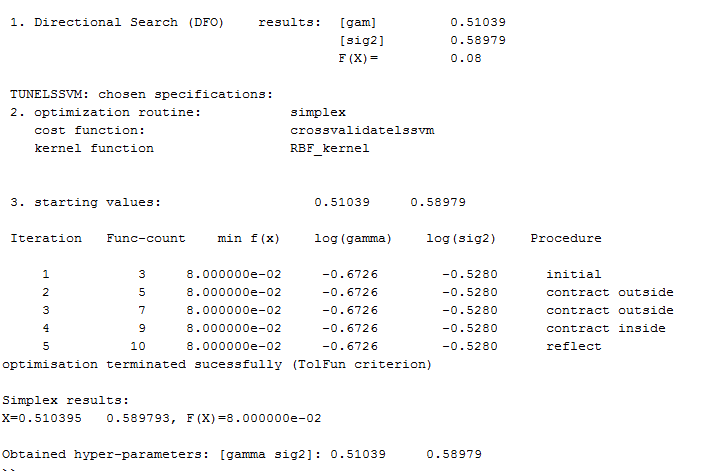
\includegraphics[width=\textwidth]{../Figures/breast_DS_simp}
		\caption{DS and simplex}
	\end{subfigure}
	\caption{Different tuning methods}
	
\end{figure}

\textbf{5. Judge your final model. Is the methodology perfectly suited for this data-set?}

\subsubsection{Breast Cancer Dataset}

\textbf{1. Look at the plotted data. What seems to be important properties of the data?}\\

The datasets are completely intertwined.

\begin{figure}[H]
	\centering
	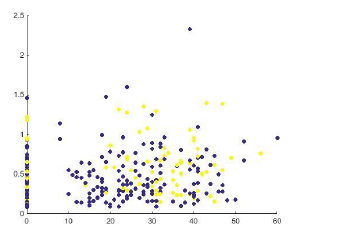
\includegraphics[scale=0.4]{../Figures/diabetes_viz}
	\caption{viz of diabetes }
\end{figure}
\textbf{2. Try a linear model. Do you think it’s sufficient?}\\
\begin{figure}[H]
	\centering
	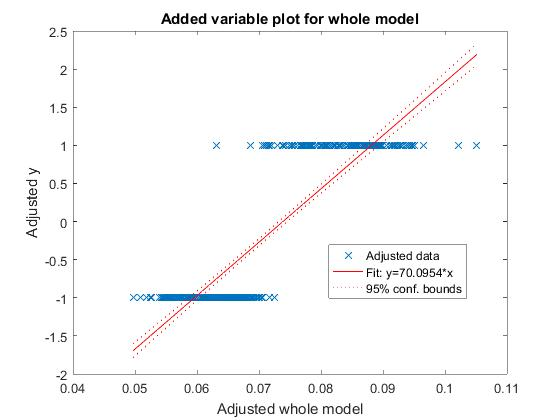
\includegraphics[scale=0.4]{../Figures/diabetes_linear}
	\caption{viz of diabetes }
\end{figure}
\textbf{3. Try the RBF kernel and tune its parameter. Is the tuning acceptable? Run several times the routine tunelssvm. Do the tuned parameters gam and sig2 change? What about the performance?}\\
\begin{figure}[H]
	\begin{subfigure}[b]{0.4\textwidth}
		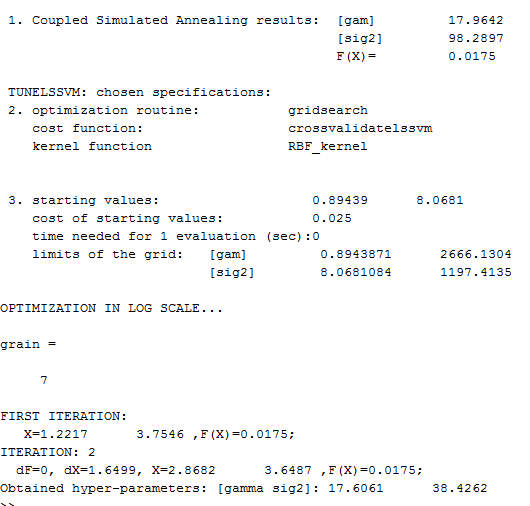
\includegraphics[width=\textwidth]{../Figures/diabetes_CSA_grid}
		\caption{CSA and gridsearch}
	\end{subfigure}
	%
	\begin{subfigure}[b]{0.4\textwidth}
		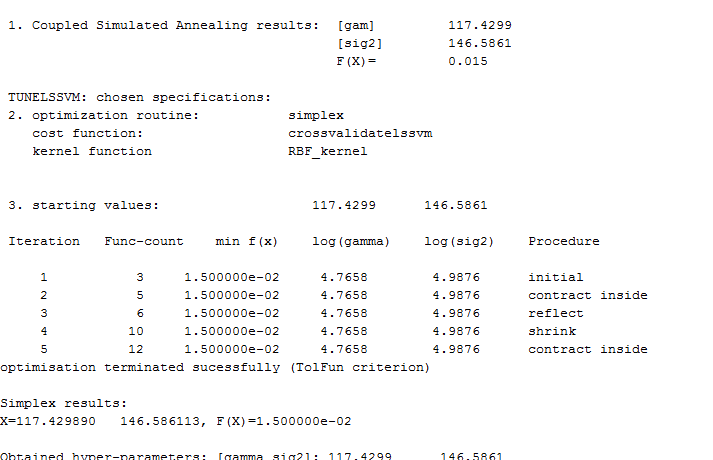
\includegraphics[width=\textwidth]{../Figures/diabetes_CSA_simp}
		\caption{CSA and simplex}
	\end{subfigure}
	%
	\begin{subfigure}[b]{0.4\textwidth}
		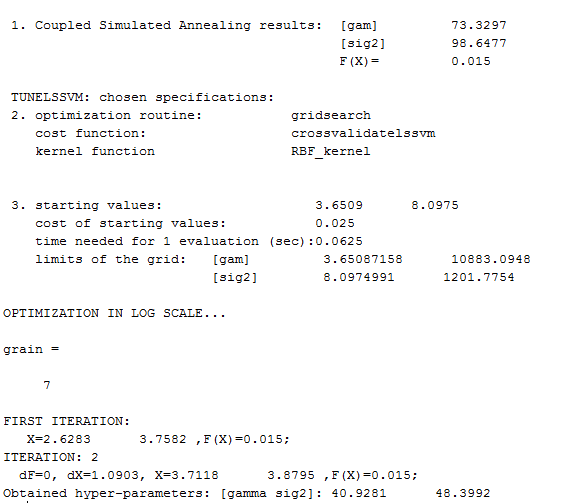
\includegraphics[width=\textwidth]{../Figures/diabetes_DS_grid}
		\caption{DS and grid search}
	\end{subfigure}
	%
	\begin{subfigure}[b]{0.4\textwidth}
		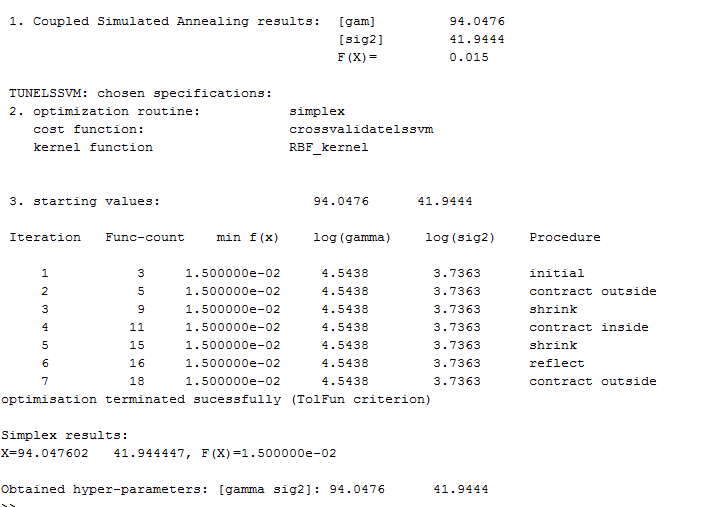
\includegraphics[width=\textwidth]{../Figures/diabetes_DS_simp}
		\caption{DS and simplex}
	\end{subfigure}
	\caption{Different tuning methods}
	
\end{figure}

\section{Assignment 2}

\subsection{The support vector machine for regression}
SVMs can also be used to solve regression problems. In the following exercises that means modeling 20 data points. The higher the e values the less support vectors are used. Sparsity comes into play when you show the model new data. A model where the bound is inf and the e is equal to 0 will generalize very poorly even if it fits well the validation set. In the default setup you do not have sparseness. All data points are support vectors, which takes away the benefit of SVMs, non-zero support vectors describing the model instead of all data points. \\  
\textbf{Construct a data-set of around 20 data-points. Which kernel is best suited for your data-set?}\\
The initial 20 point dataset was created using the uiregress interface. The best kernel was the Exponential RBF. 
\begin{figure}[H]
	\centering
	\includegraphics[scale=0.4]{../Figures/urigress_best}
	\caption{20 Data points }
\end{figure}

The the higher the e value the further it is from being a good model. 
\begin{figure}[H]
	\begin{subfigure}[b]{0.4\textwidth}
		\includegraphics[width=\textwidth]{../Figures/linear_1}
		\caption{e = .1}
	\end{subfigure}
	%
	\begin{subfigure}[b]{0.4\textwidth}
		\includegraphics[width=\textwidth]{../Figures/linear_25}
		\caption{e =.25}
	\end{subfigure}
	%
	\begin{subfigure}[b]{0.4\textwidth}
		\includegraphics[width=\textwidth]{../Figures/linear_5}
		\caption{e = .5}
	\end{subfigure}
	%
	\begin{subfigure}[b]{0.4\textwidth}
		\includegraphics[width=\textwidth]{../Figures/linear_urigress}
		\caption{default values}
	\end{subfigure}
	\caption{Different values of e}
	
\end{figure}

\begin{figure}[H]
	\begin{subfigure}[b]{0.4\textwidth}
		\includegraphics[width=\textwidth]{../Figures/linear_b_01}
		\caption{bound = 0.01}
	\end{subfigure}
	%
	\begin{subfigure}[b]{0.4\textwidth}
		\includegraphics[width=\textwidth]{../Figures/linear_b_1}
		\caption{bound = 0.1}
	\end{subfigure}
	%
	\begin{subfigure}[b]{0.4\textwidth}
		\includegraphics[width=\textwidth]{../Figures/linear_b_11}
		\caption{bound = 1}
	\end{subfigure}
	%
	\begin{subfigure}[b]{0.4\textwidth}
		\includegraphics[width=\textwidth]{../Figures/linear_b_10}
		\caption{bound = 10}
	\end{subfigure}
	%
	\begin{subfigure}[b]{0.4\textwidth}
		\includegraphics[width=\textwidth]{../Figures/linear_b_100}
		\caption{bound = 100}
	\end{subfigure}
	\caption{Different values for the bound}
	
\end{figure}

\subsection{A Simple Example: Sum of Cosines}

\textbf{Do you think there is one pair of optimal hyper-parameters?}
The model was very constrained with the original parameters. Due to its linear nature sig2 was too high. Reducing both parameters gave a better fit. 

\begin{figure}[H]
	\begin{subfigure}[b]{0.4\textwidth}
		\includegraphics[width=\textwidth]{../Figures/test_sig_gam_arb}
		\caption{arbitrary sigma and gamma, 100 and 1.0}
	\end{subfigure}
	%
	\begin{subfigure}[b]{0.4\textwidth}
		\includegraphics[width=\textwidth]{../Figures/sig_gama_50_1}
		\caption{gamma = 50, sigma = 0.1}
	\end{subfigure}
	%
	\begin{subfigure}[b]{0.4\textwidth}
		\includegraphics[width=\textwidth]{../Figures/sig_gama_25_01}
		\caption{gamma = 25, sigma = 0.01}
	\end{subfigure}
	%
	\begin{subfigure}[b]{0.4\textwidth}
		\includegraphics[width=\textwidth]{../Figures/sig_gama_200_1}
		\caption{gamma = 200 and sigma = 10}
	\end{subfigure}
	\caption{Different values for sigma and gamma}
	
\end{figure}

\subsection{Hyper-parameter Tuning}

\textbf{
What can you say about the values of the hyperparameters
and the results? What is the difference between 'simplex' and 'gridsearch'? Is there any significant deviation in results?
Which method is faster and why?}\\

The hyperparameters vary in a pretty tight range between sigma = .05-.11 to gamma = 500-1000. The simplex is an algorithm while the gridsearch is brute force. Although they happened to fall within similar ranges. The fastest is csa and simplex together because these are algorithms that go about parameter tunning methodically. The results of all methods are similar but the DS and gridsearch take a lot of time. 

\subsection{Application of the Bayesian Framework}
A decreasing of the sig2 value increases the probability of the data to belong to the positive class. Increasing of the gamma parameter allowed for more misclassification. If a point falls into a blue area it is more likely to be a negative class and if it falls in into a purple area it is more likely to be positive. Lowering sigma gives you a more rigid boundary and lowers the chance of misclassification. Raising gamma gives you a fuzzier decision boundary.
\begin{figure}[H]
	\begin{subfigure}[b]{0.4\textwidth}
		\includegraphics[width=\textwidth]{../Figures/test_data_bayes}
	\end{subfigure}
	%
	\begin{subfigure}[b]{0.4\textwidth}
		\includegraphics[width=\textwidth]{../Figures/dig_sig}
	\end{subfigure}
	%
	\begin{subfigure}[b]{0.4\textwidth}
		\includegraphics[width=\textwidth]{../Figures/gam_sig_dif}

	\end{subfigure}
	%
	\begin{subfigure}[b]{0.4\textwidth}
		\includegraphics[width=\textwidth]{../Figures/gamma_50_bayes}

	\end{subfigure}
	
\end{figure}

\begin{figure}[H]
	\begin{subfigure}[b]{0.4\textwidth}
		\includegraphics[width=\textwidth]{../Figures/sig_1_bayes}
	\end{subfigure}
	%
	\begin{subfigure}[b]{0.4\textwidth}
		\includegraphics[width=\textwidth]{../Figures/sig_01_bayes}
	\end{subfigure}
	%
	\begin{subfigure}[b]{0.4\textwidth}
		\includegraphics[width=\textwidth]{../Figures/sig_2_bayes}
		
	\end{subfigure}
\end{figure}

\textbf{Can you think of a similar way to do input selection by
using the crossvalidate function instead of the Bayesian framework?}

 It possible by creating all possible variable combinations and crossvalidating all models to score the MSE. It would take a long time be prohibitively time consuming. 
\subsection{Robust Regression}
A model of with outlier in the data will cause noise in the model. It will cause the model to be bais by their values. MAE is used because it is less sensitive to outliers. 
\begin{figure}[H]
	\centering
	\includegraphics[scale=0.4]{../Figures/robust}
\end{figure}

\subsection{Time-series Prediction}
SVM can also work on predicted time-series sequences. 

\subsection{Sante Fe laser Data}

\begin{figure}[H]
	\centering
	\includegraphics[scale=.5]{../Figures/sante_fe}
\end{figure}

Yes this seems like a good choice. The model lags but can still predict pretty well.

If you used a validation set to optimize you would get autocorrelation. 
\section{Assignment 3}

This section will discuss unsupervised learning.

\subsection{PCA}

\begin{figure}[H]
	\begin{subfigure}[b]{0.4\textwidth}
		\includegraphics[width=\textwidth]{../Figures/linaer_3}
		\caption{3 components}
	\end{subfigure}
	%
	\begin{subfigure}[b]{0.4\textwidth}
		\includegraphics[width=\textwidth]{../Figures/kernal_3}
		\caption{3 components}
	\end{subfigure}
	%
	\begin{subfigure}[b]{0.4\textwidth}
		\includegraphics[width=\textwidth]{../Figures/kernel_9}
		\caption{9 components}
	\end{subfigure}
	%
	\begin{subfigure}[b]{0.4\textwidth}
		\includegraphics[width=\textwidth]{../Figures/kernal_20}
		\caption{20 components}
\end{subfigure}		
\end{figure}
\textbf{Kernel PCA can be used for feature extraction, denoising, dimensionality reduction and density estimation. Can you describe what's happening with the denoising if you increase the number of principal components? What is the difference with linear PCA? How many principal components can you obtain with kernel PCA? and
with linear PCA? Can you think of a technique to tune the number of components and the kernel hyper-parameter?}\\

As the number of PC increased the model started to look better. However after a certain amount you start to overfit. Linear PCA does not work for this data at all. Around 3 components we start to get a model that gets really well. The none linear character of that is being captures. The linear PCA is a dimension reduction technique that can have as many components as dimensions. A kernel PCA can have infinite number of dimensions because it takes place in the kernel space. 

\subsection{Handwritten Digit Denoising}

\textbf{This data-set consists of features of handwritten numerals (0 to 9) extracted from a collection of Dutch utility maps. Try the sample script on Toledo and explain what you observe.}\\

First line is the original data. The second has noice added to it. The rows that follow show the PCA's trying to remove the noise. As you can see the kernel PCA does much better than the liner one. 
\begin{figure}[H]
	\begin{subfigure}[b]{0.5\textwidth}
		\includegraphics[width=\textwidth]{../Figures/hand}
		\caption{Kernel PCA}
	\end{subfigure}
	%
	\begin{subfigure}[b]{0.5\textwidth}
		\includegraphics[width=\textwidth]{../Figures/linear_hand}
		\caption{Linear PCA}
	\end{subfigure}
	
\end{figure}

\subsection{Spectral Clustering}

\textbf{What is the difference with classification?}
Classification is a supervised method. This means that it is trained on data where the "answer" is known. Data that already has a set of predicitions. Clustering estimates which class a particular points belongs into.
\begin{figure}[H]
	\begin{subfigure}[b]{0.4\textwidth}
		\includegraphics[width=\textwidth]{../Figures/sig001}
		\caption{sig = 0.001}
	\end{subfigure}
	%
	\begin{subfigure}[b]{0.4\textwidth}
		\includegraphics[width=\textwidth]{../Figures/sig01}
		\caption{sig = 0.01}
	\end{subfigure}
	%
	\begin{subfigure}[b]{0.4\textwidth}
		\includegraphics[width=\textwidth]{../Figures/sig005}
		\caption{sig = 0.005}
	\end{subfigure}
		\begin{subfigure}[b]{0.4\textwidth}
			\includegraphics[width=\textwidth]{../Figures/sig01m}
		\end{subfigure}
\end{figure}

The low sigma classifies perfectly in one ring. The higher sigma goes the more misclassification is allowed. Eventually though when it goes high enough the other ring gets classified perfectly.

\begin{figure}[H]
	\begin{subfigure}[b]{0.4\textwidth}
		\includegraphics[width=\textwidth]{../Figures/sig001s}
		\caption{sig = 0.001}
	\end{subfigure}
	%
	\begin{subfigure}[b]{0.4\textwidth}
		\includegraphics[width=\textwidth]{../Figures/sig01s}
		\caption{sig = 0.01}
	\end{subfigure}
	%
	\begin{subfigure}[b]{0.4\textwidth}
		\includegraphics[width=\textwidth]{../Figures/sig005s}
		\caption{sig = 0.005}
	\end{subfigure}
\end{figure}

\subsection{Fixed Size LS-SVM}

\textbf{ What is the influence of the chosen sig2?}

Fixed sized SVM has a bases of two ideas. Using the primal-dual formulation of LS-SVM and secondly to select support vectors actively. When sigma decreases the points start to move towards a single side. When sigma increase the points tend to spread out.

\begin{figure}[H]
	\begin{subfigure}[b]{0.4\textwidth}
		\includegraphics[width=\textwidth]{../Figures/sig05aprox}
		\caption{sig = 0.05}
	\end{subfigure}
	%
	\begin{subfigure}[b]{0.4\textwidth}
		\includegraphics[width=\textwidth]{../Figures/sig100aprox}
		\caption{sig = 150}
	\end{subfigure}
\end{figure}



\end{document}